\documentclass[../cellseek_paper.tex]{subfiles}

\begin{document}

\section{Results}

We evaluated CellSeek against TrackMate \cite{tinevez2017trackmate} configured with both Laplacian-of-Gaussian (LoG) detector and a state-of-the-art deep learning-based detector, StarDist \cite{schmidt2018cell}. Tracking was performed using the simple LAP tracker \cite{jaqaman2008robust} in all cases.

\subsect  \begin{tabular}{lccc}
  \toprule
  \textbf{Dataset}   & \textbf{CellSeek TRA} & \textbf{TrackMate TRA} & \textbf{Processing Time} \\
  \midrule
  DIC-HeLa           & 0.842 ± 0.031         & 0.856 ± 0.028          & 4.2min vs 52min          \\
  Fluo-N2DH          & 0.891 ± 0.022         & 0.903 ± 0.019          & 3.8min vs 41min          \\
  Custom-Bacteria    & 0.765 ± 0.045         & 0.771 ± 0.041          & 5.1min vs 73min          \\
  Custom-Fibroblasts & 0.723 ± 0.052         & 0.748 ± 0.039          & 6.3min vs 89min          \\
  \bottomrule
\end{tabular}ity Analysis: CellSeek vs. TrackMate}

To quantify the usability advantage of CellSeek, we conducted a comparative workflow analysis examining the steps, decisions, and expertise required to achieve tracking results across different platforms. We analyzed three experimental scenarios representing common biological applications:

\textbf{Scenario 1:} Fluorescent nuclei in HeLa cells (2D, 100 frames)

\textbf{Scenario 2:} Phase-contrast fibroblasts with high cell density (2D, 200 frames)

\textbf{Scenario 3:} Bacterial microcolonies in brightfield (2D, 150 frames)

\subsubsection{TrackMate Workflow Complexity}

TrackMate analysis requires navigating a complex decision tree with numerous parameter optimization steps:

\begin{enumerate}
  \item \textbf{Detector Selection}: Choose between LoG, DoG, StarDist \cite{schmidt2018cell}, or Cellpose \cite{stringer2021cellpose} detectors, each with different strengths and parameter requirements
  \item \textbf{Detection Parameter Tuning}: Optimize spot diameter, threshold values, quality filters, and preprocessing options
  \item \textbf{Feature Calculation}: Select appropriate features for tracking (intensity, morphology, texture)
  \item \textbf{Tracker Configuration}: Choose tracking algorithm (LAP \cite{jaqaman2008robust}, simple, manual) and configure linking parameters
  \item \textbf{Linking Optimization}: Adjust linking max distance, gap-closing parameters, splitting/merging costs
  \item \textbf{Post-processing}: Apply track filters, validate results, and potentially iterate through previous steps
\end{enumerate}

This workflow requires deep understanding of computer vision concepts, familiarity with cellular morphology, and experience with parameter optimization strategies. Users must make dozens of interdependent decisions with limited guidance, often requiring multiple iterations to achieve acceptable results.

\subsubsection{CellSeek Workflow Simplicity}

In contrast, CellSeek dramatically simplifies the tracking workflow:

\begin{enumerate}
  \item \textbf{Data Import}: Drag-and-drop loading of microscopy data
  \item \textbf{Initial Segmentation}: Automatic first-frame processing with Cellpose-SAM
  \item \textbf{Interactive Correction}: Optional point-and-click editing using SAM's intuitive interface (typically 2-3 interactions per frame for correction)
  \item \textbf{Tracking Initiation}: Single click to start automated tracking
  \item \textbf{Progress Monitoring}: Watch side-by-side comparison as tracking proceeds
  \item \textbf{Selective Intervention}: Intervene at any frame to correct errors using SAM tools
\end{enumerate}

The CellSeek workflow eliminates the need for parameter optimization, reduces the decision burden by over 90\%, and provides intuitive visual feedback throughout the process. The integration of SAM's interactive segmentation capabilities allows users to correct errors with natural point-and-click interactions rather than complex parameter adjustments.

\subsubsection{Expertise Requirement Comparison}

The expertise requirements for both platforms reveal stark differences:

\begin{table}[H]
  \centering
  \caption{Expertise requirements comparison}
  \begin{tabular}{lcc}
    \toprule
    \textbf{Required Knowledge} & \textbf{TrackMate} & \textbf{CellSeek} \\
    \midrule
    Computer vision concepts    & Extensive          & Minimal           \\
    Parameter optimization      & Required           & Eliminated        \\
    Cellular morphology         & Expert-level       & Basic             \\
    Software navigation         & Complex            & Intuitive         \\
    Error debugging             & Advanced           & Guided            \\
    \bottomrule
  \end{tabular}
\end{table}

CellSeek reduces the expertise barrier by providing guided workflows, visual feedback, and intuitive correction tools that require only basic biological knowledge rather than specialized computational skills.

\subsection{Model Generalizability Across Diverse Microscopy Techniques}

To demonstrate the broad applicability of CellSeek, we evaluated the system across twelve diverse examples spanning multiple microscopy techniques and cell types without any parameter modifications or retraining. Figure \ref{fig:generalization_examples} showcases segmentation results across this diverse collection, highlighting the model's robust generalization capabilities.

\begin{figure}[H]
  \centering
  \begin{subfigure}{0.23\textwidth}
    \centering
    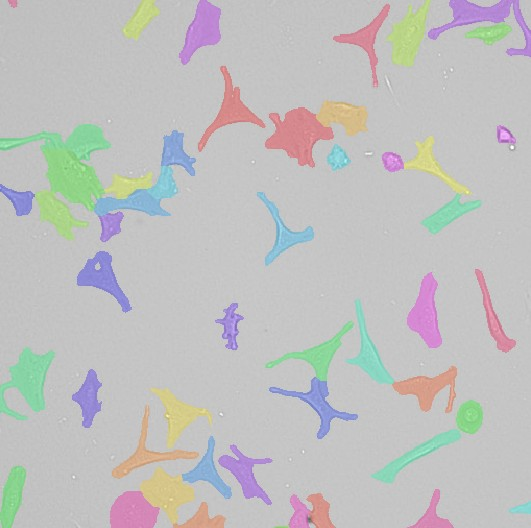
\includegraphics[width=\textwidth,height=3cm]{images/examples/fibroblast_segmented.jpg}
    \caption{\footnotesize BF Fibroblast}
    \label{fig:fibroblast}
  \end{subfigure}
  \hfill
  \begin{subfigure}{0.23\textwidth}
    \centering
    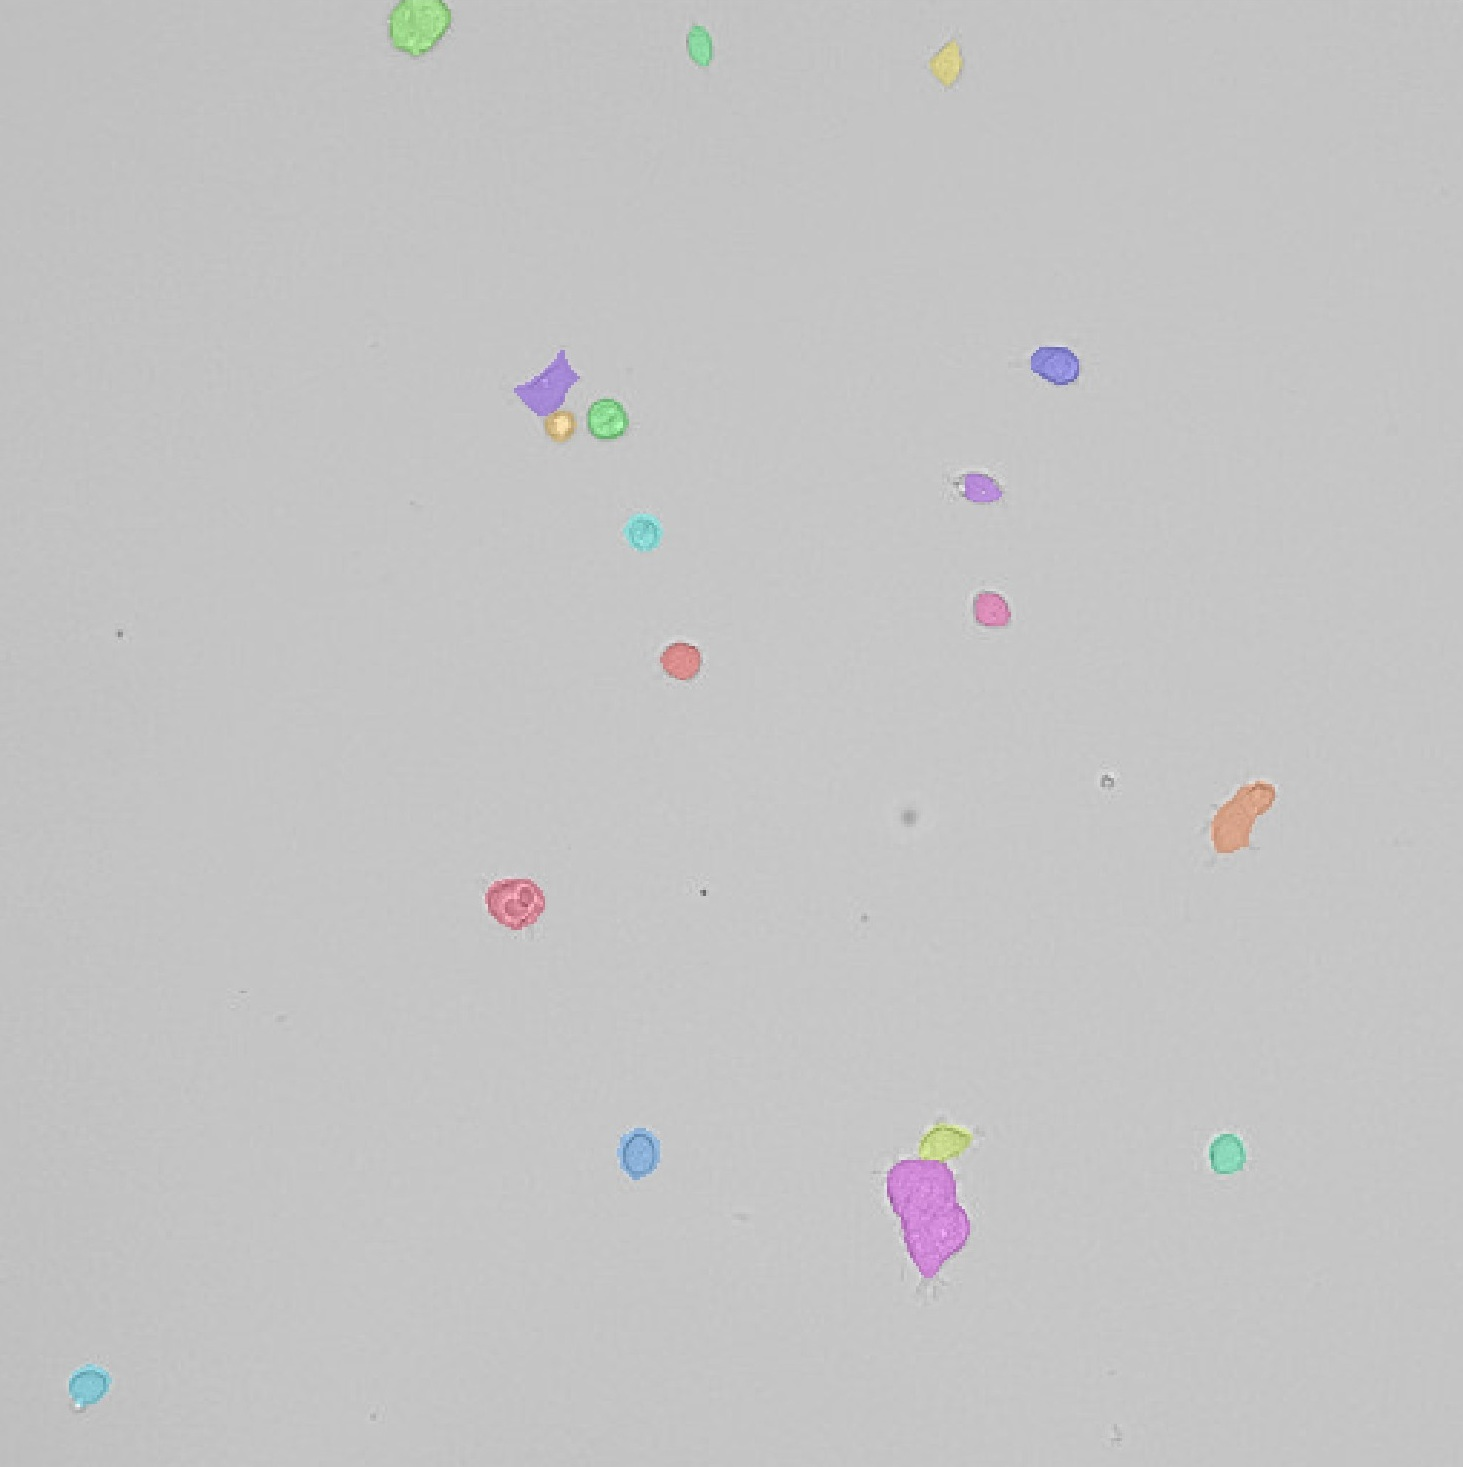
\includegraphics[width=\textwidth,height=3cm]{images/examples/293t_segmented.jpg}
    \caption{\footnotesize BF 293T}
    \label{fig:293t}
  \end{subfigure}
  \hfill
  \begin{subfigure}{0.23\textwidth}
    \centering
    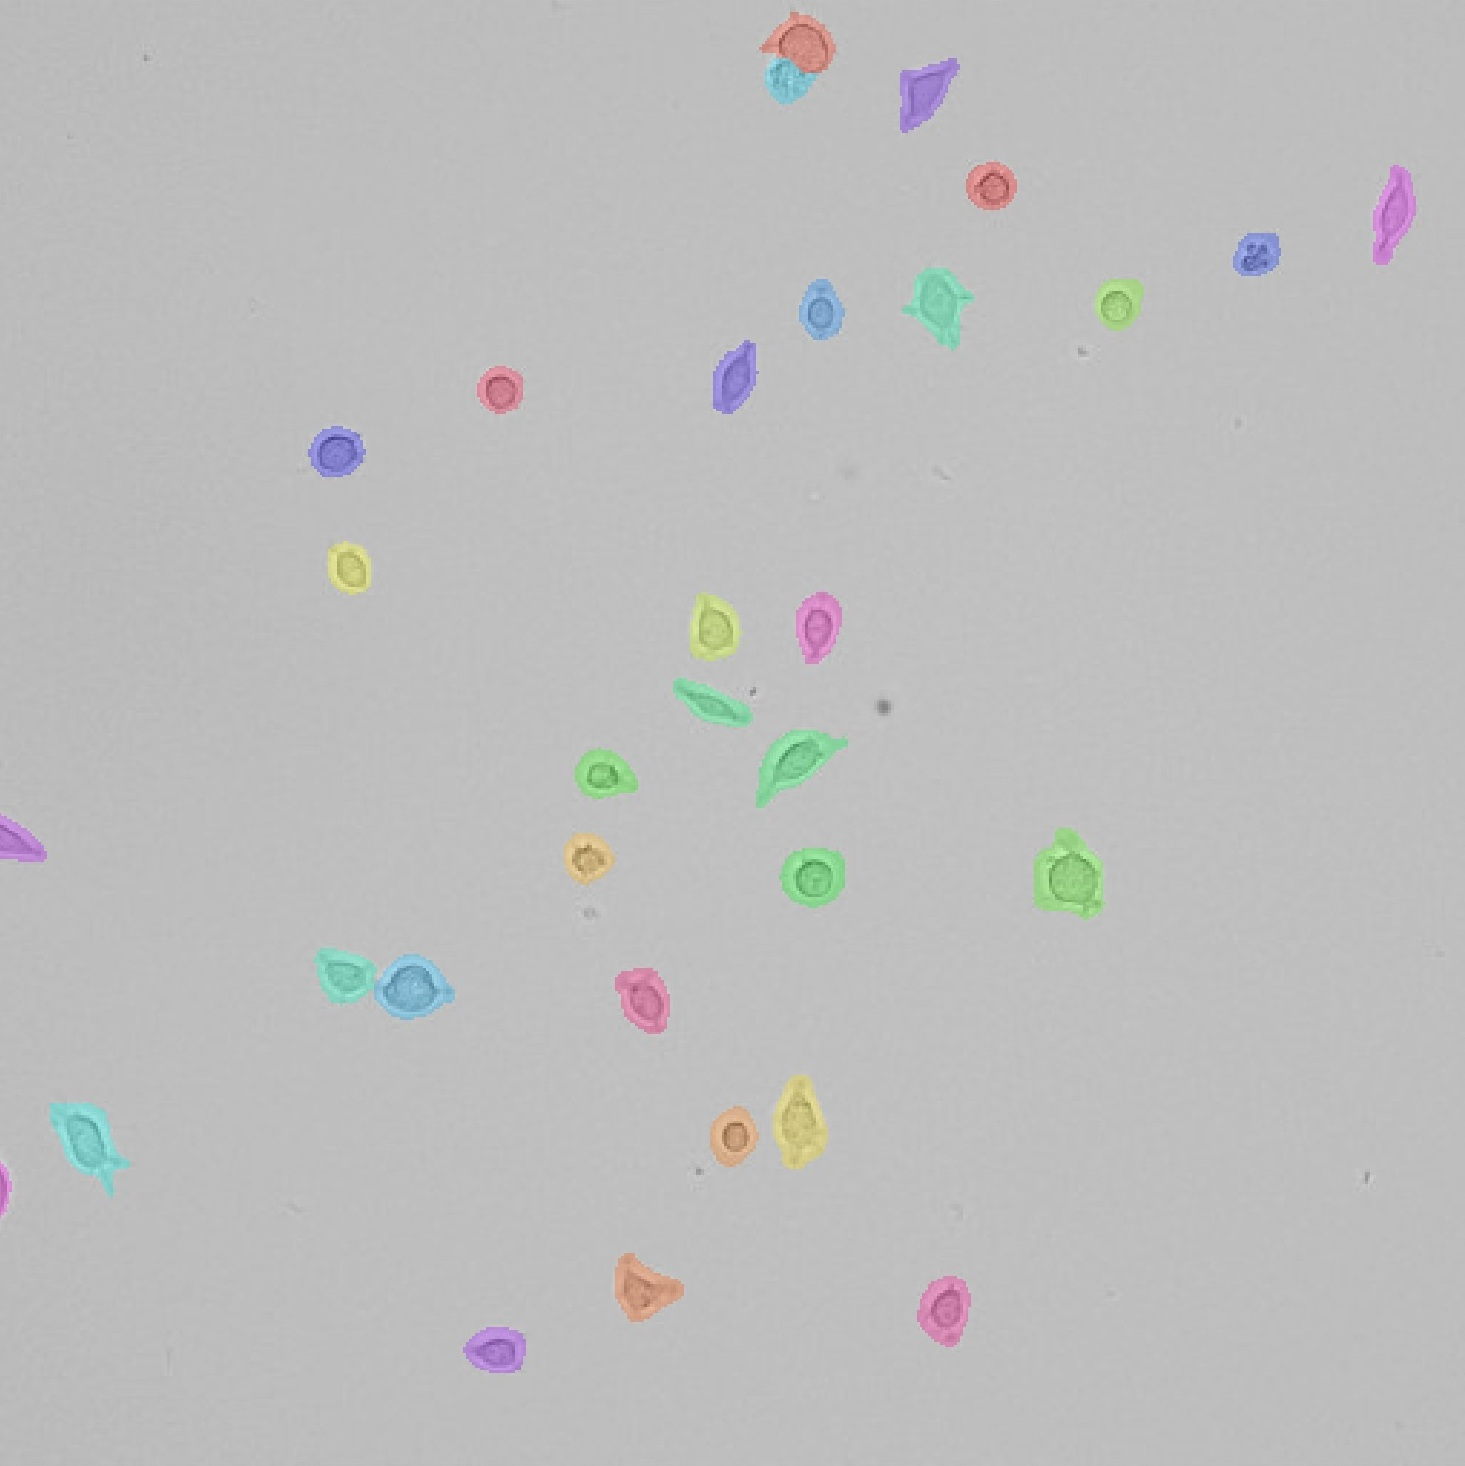
\includegraphics[width=\textwidth,height=3cm]{images/examples/mda_md_231_segmented.jpg}
    \caption{\footnotesize BF MDA-MB-231}
    \label{fig:mda}
  \end{subfigure}
  \hfill
  \begin{subfigure}{0.23\textwidth}
    \centering
    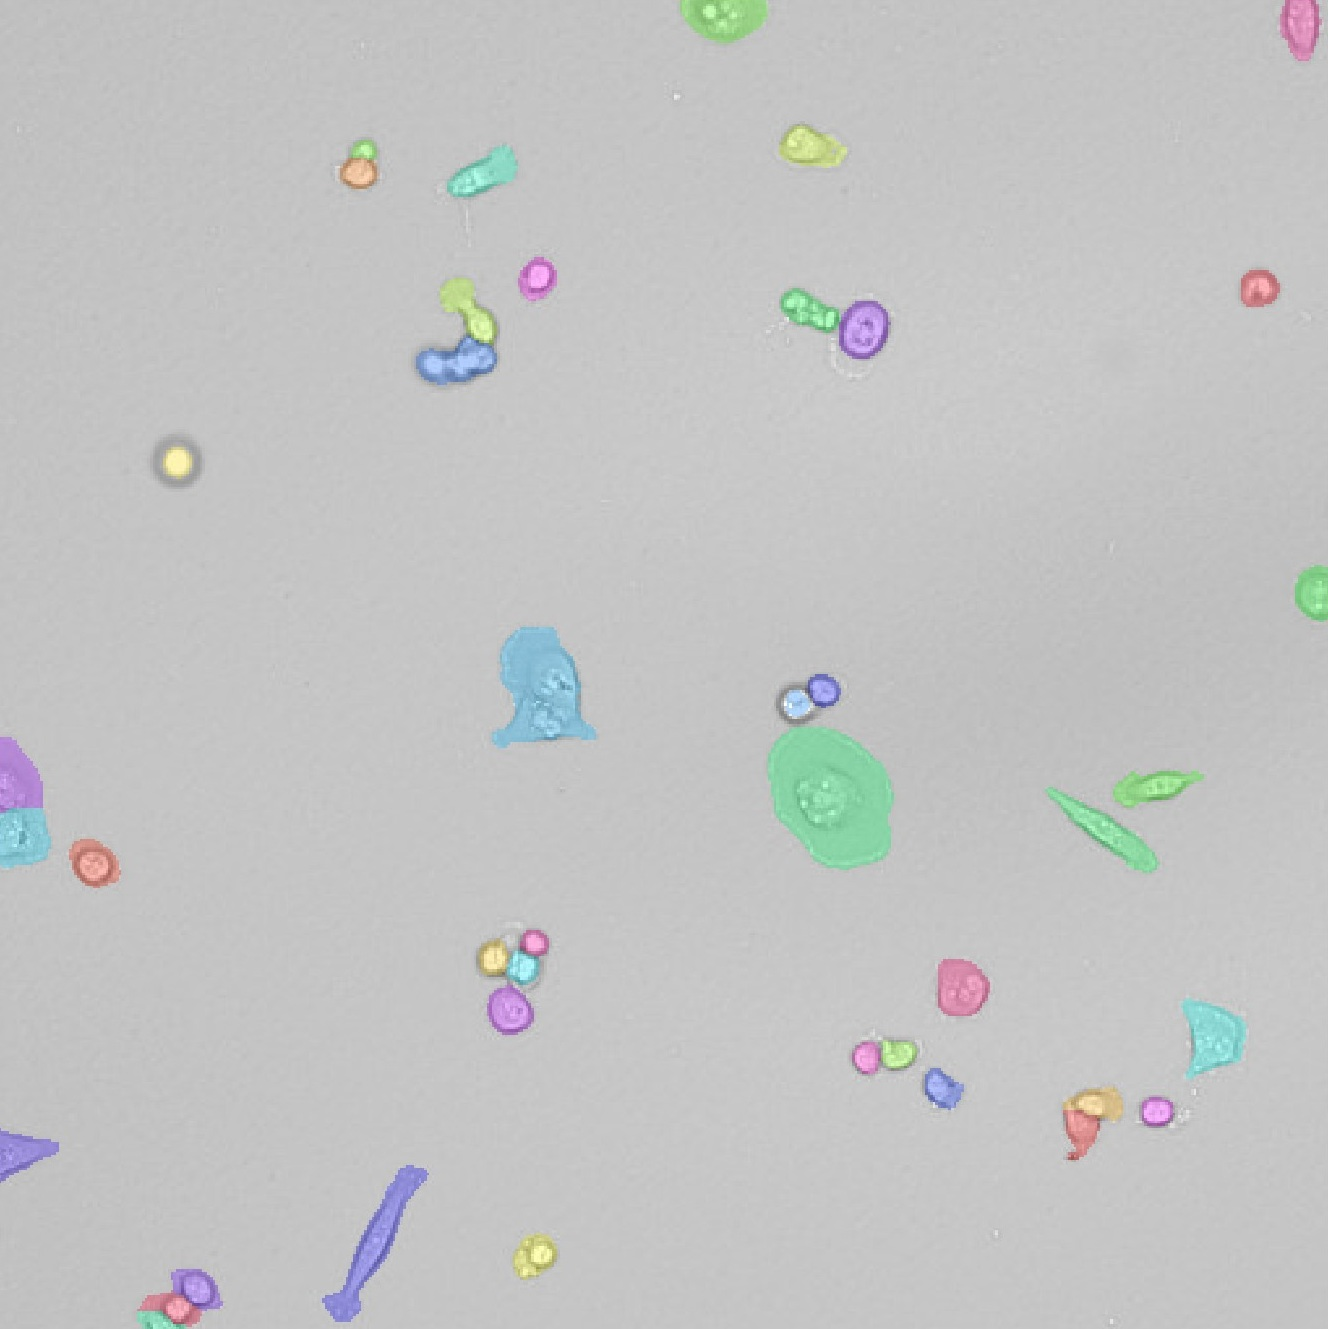
\includegraphics[width=\textwidth,height=3cm]{images/examples/cos7_segmented.jpg}
    \caption{\footnotesize BF COS-7}
    \label{fig:cos7}
  \end{subfigure}

  \vspace{0.8em}

  \begin{subfigure}{0.23\textwidth}
    \centering
    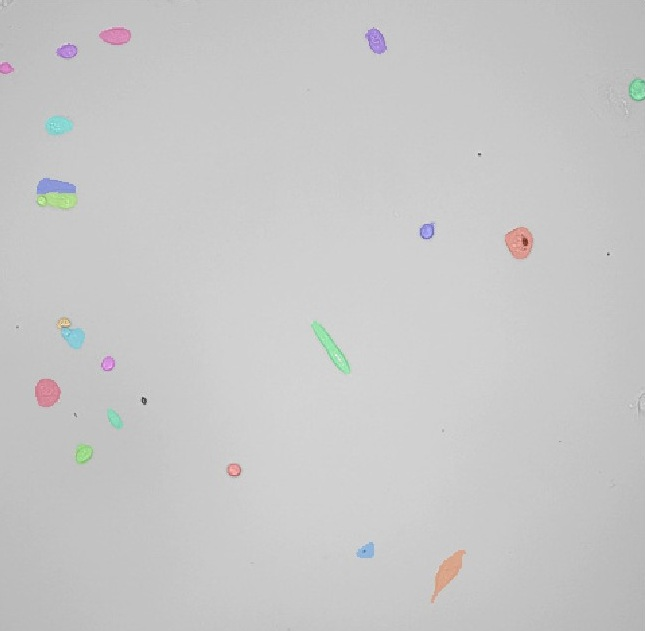
\includegraphics[width=\textwidth,height=3cm]{images/examples/myosin_segmented.jpg}
    \caption{\footnotesize BF Myosin}
    \label{fig:myosin}
  \end{subfigure}
  \hfill
  \begin{subfigure}{0.23\textwidth}
    \centering
    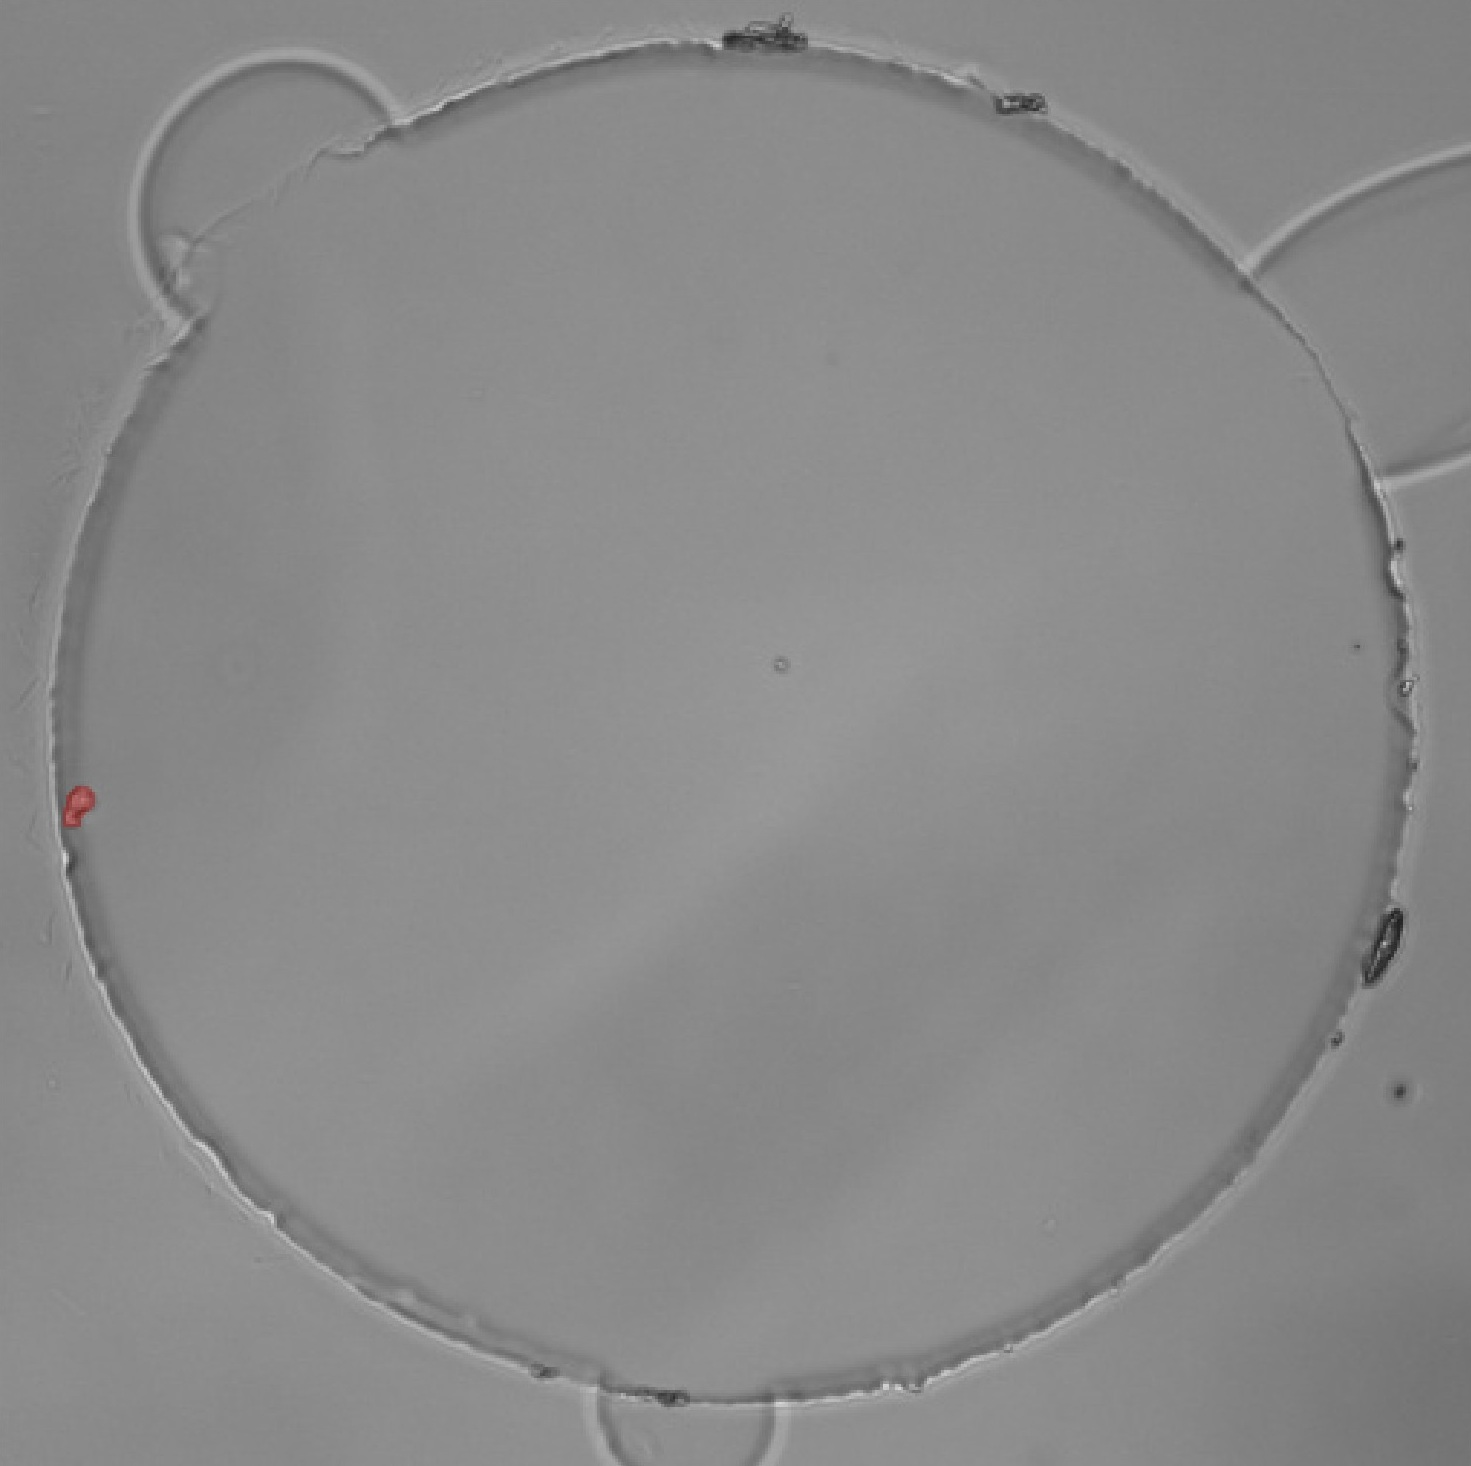
\includegraphics[width=\textwidth,height=3cm]{images/examples/hsc_segmented.jpg}
    \caption{\footnotesize BF HSC}
    \label{fig:hsc}
  \end{subfigure}
  \hfill
  \begin{subfigure}{0.23\textwidth}
    \centering
    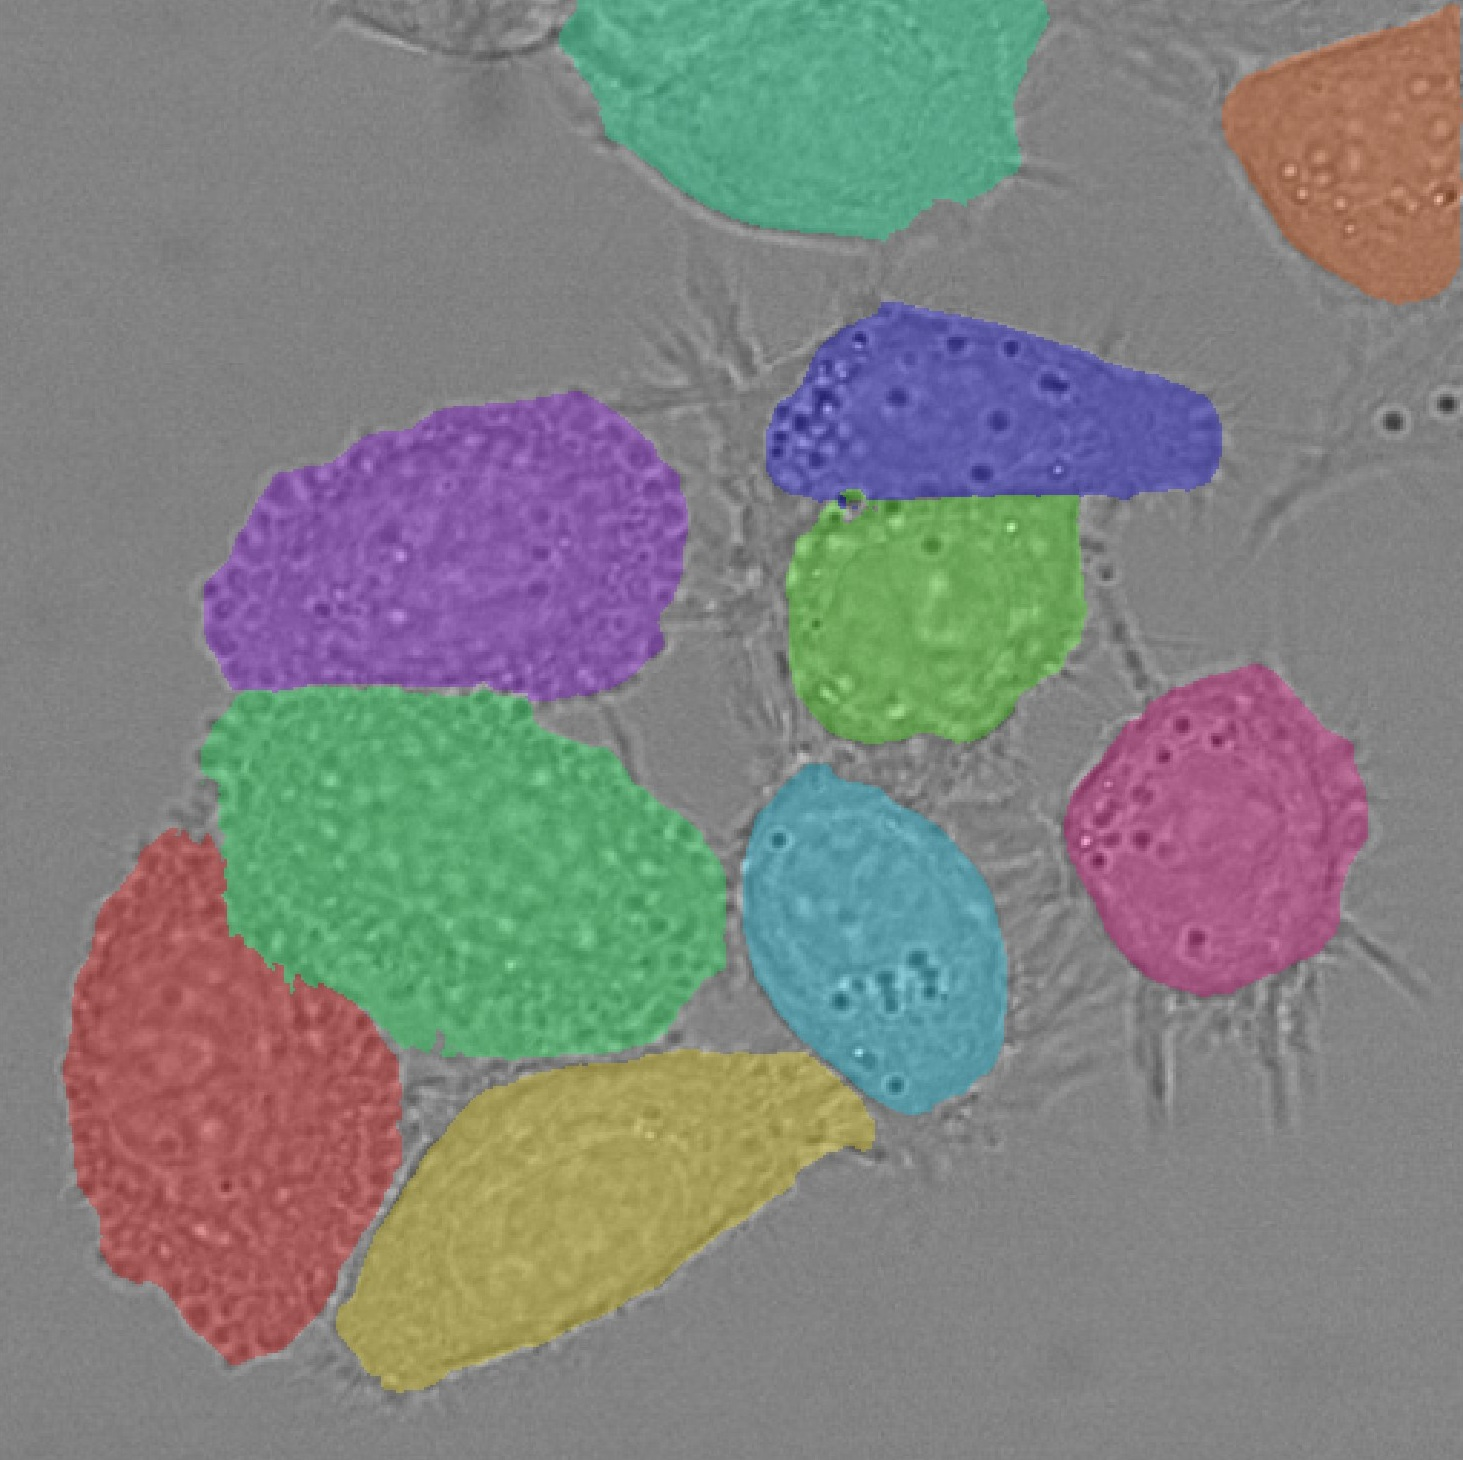
\includegraphics[width=\textwidth,height=3cm]{images/examples/hela_segmented.jpg}
    \caption{\footnotesize DIC HeLa}
    \label{fig:hela}
  \end{subfigure}
  \hfill
  \begin{subfigure}{0.23\textwidth}
    \centering
    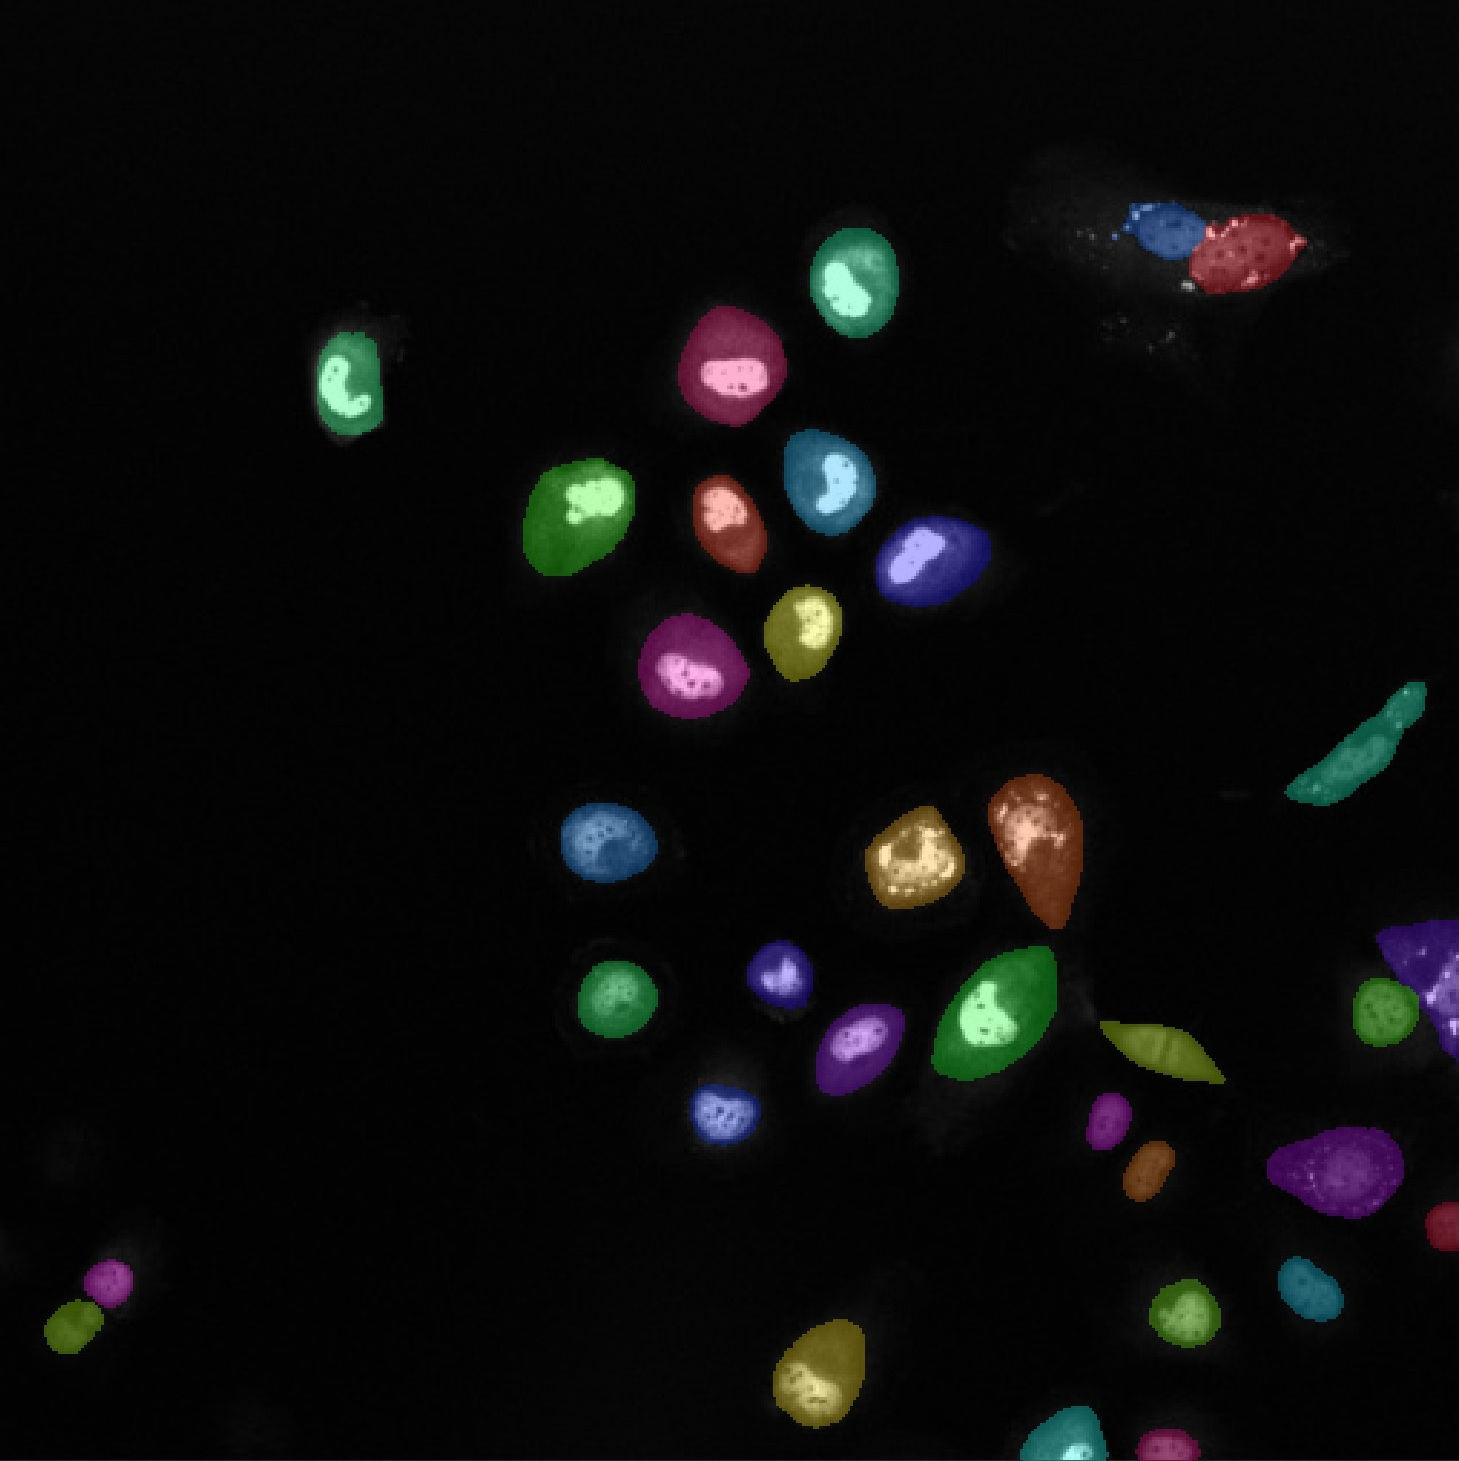
\includegraphics[width=\textwidth,height=3cm]{images/examples/huh7_segmented.jpg}
    \caption{\footnotesize Fluo Huh7}
    \label{fig:huh7}
  \end{subfigure}

  \vspace{0.8em}

  \begin{subfigure}{0.23\textwidth}
    \centering
    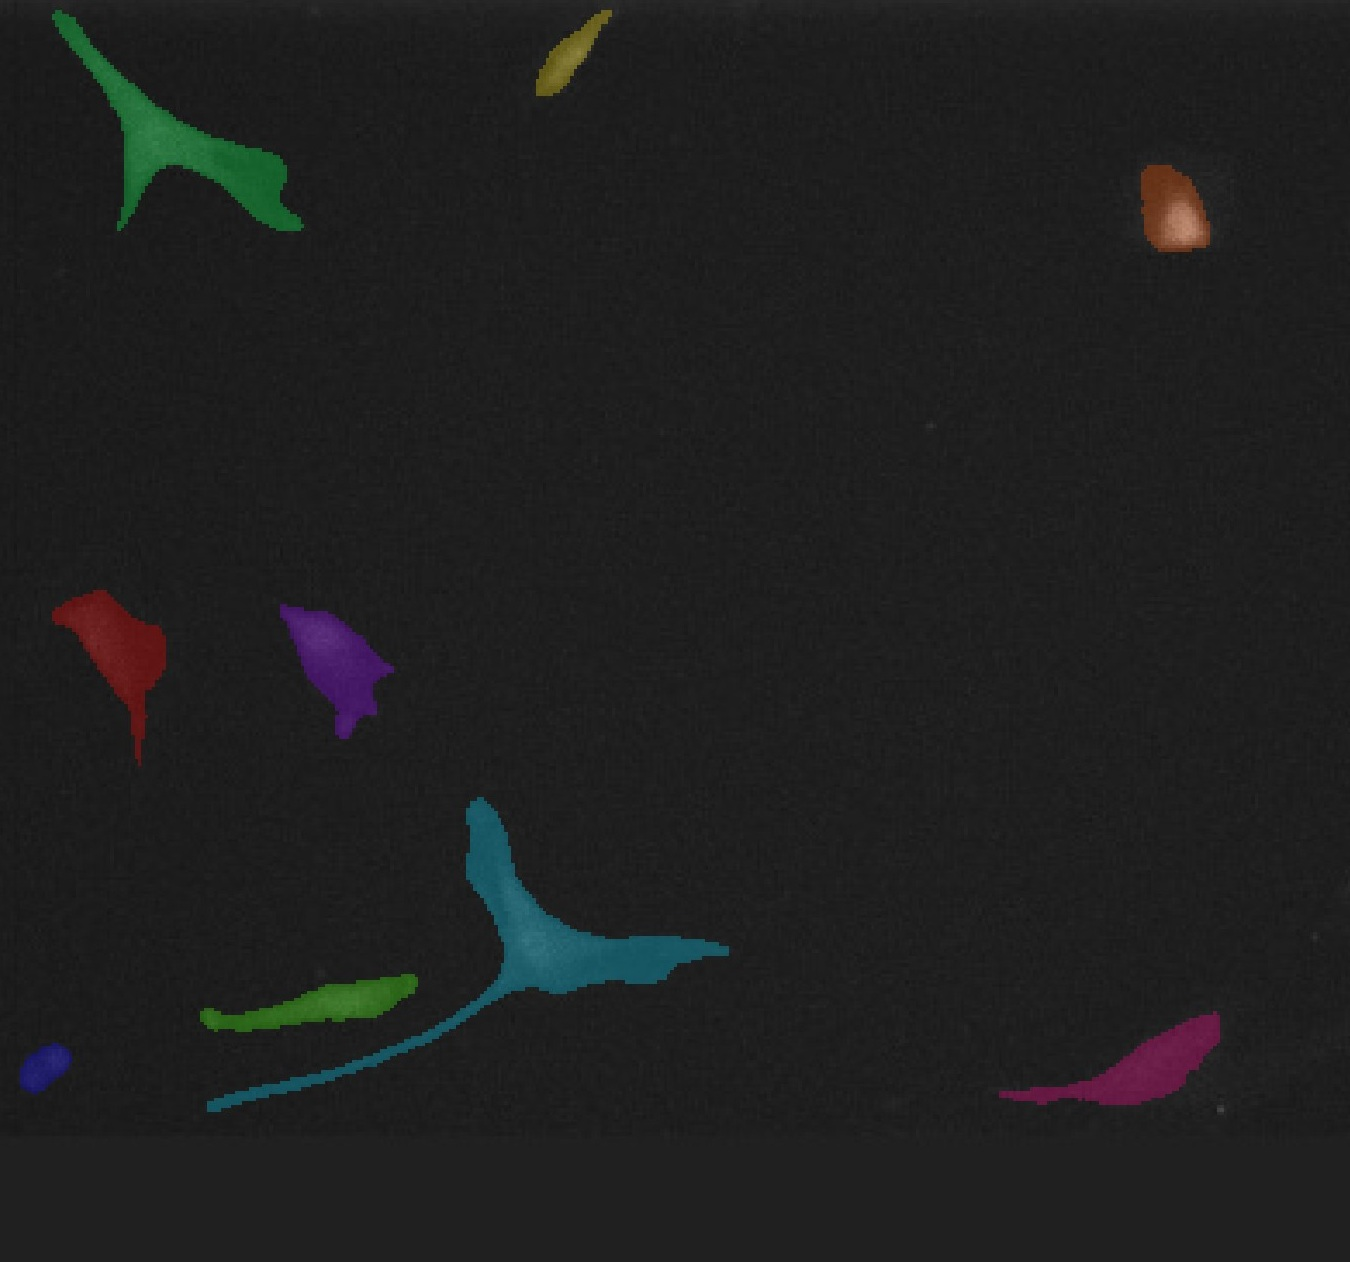
\includegraphics[width=\textwidth,height=3cm]{images/examples/msc_segmented.jpg}
    \caption{\footnotesize Fluo MSC}
    \label{fig:msc}
  \end{subfigure}
  \hfill
  \begin{subfigure}{0.23\textwidth}
    \centering
    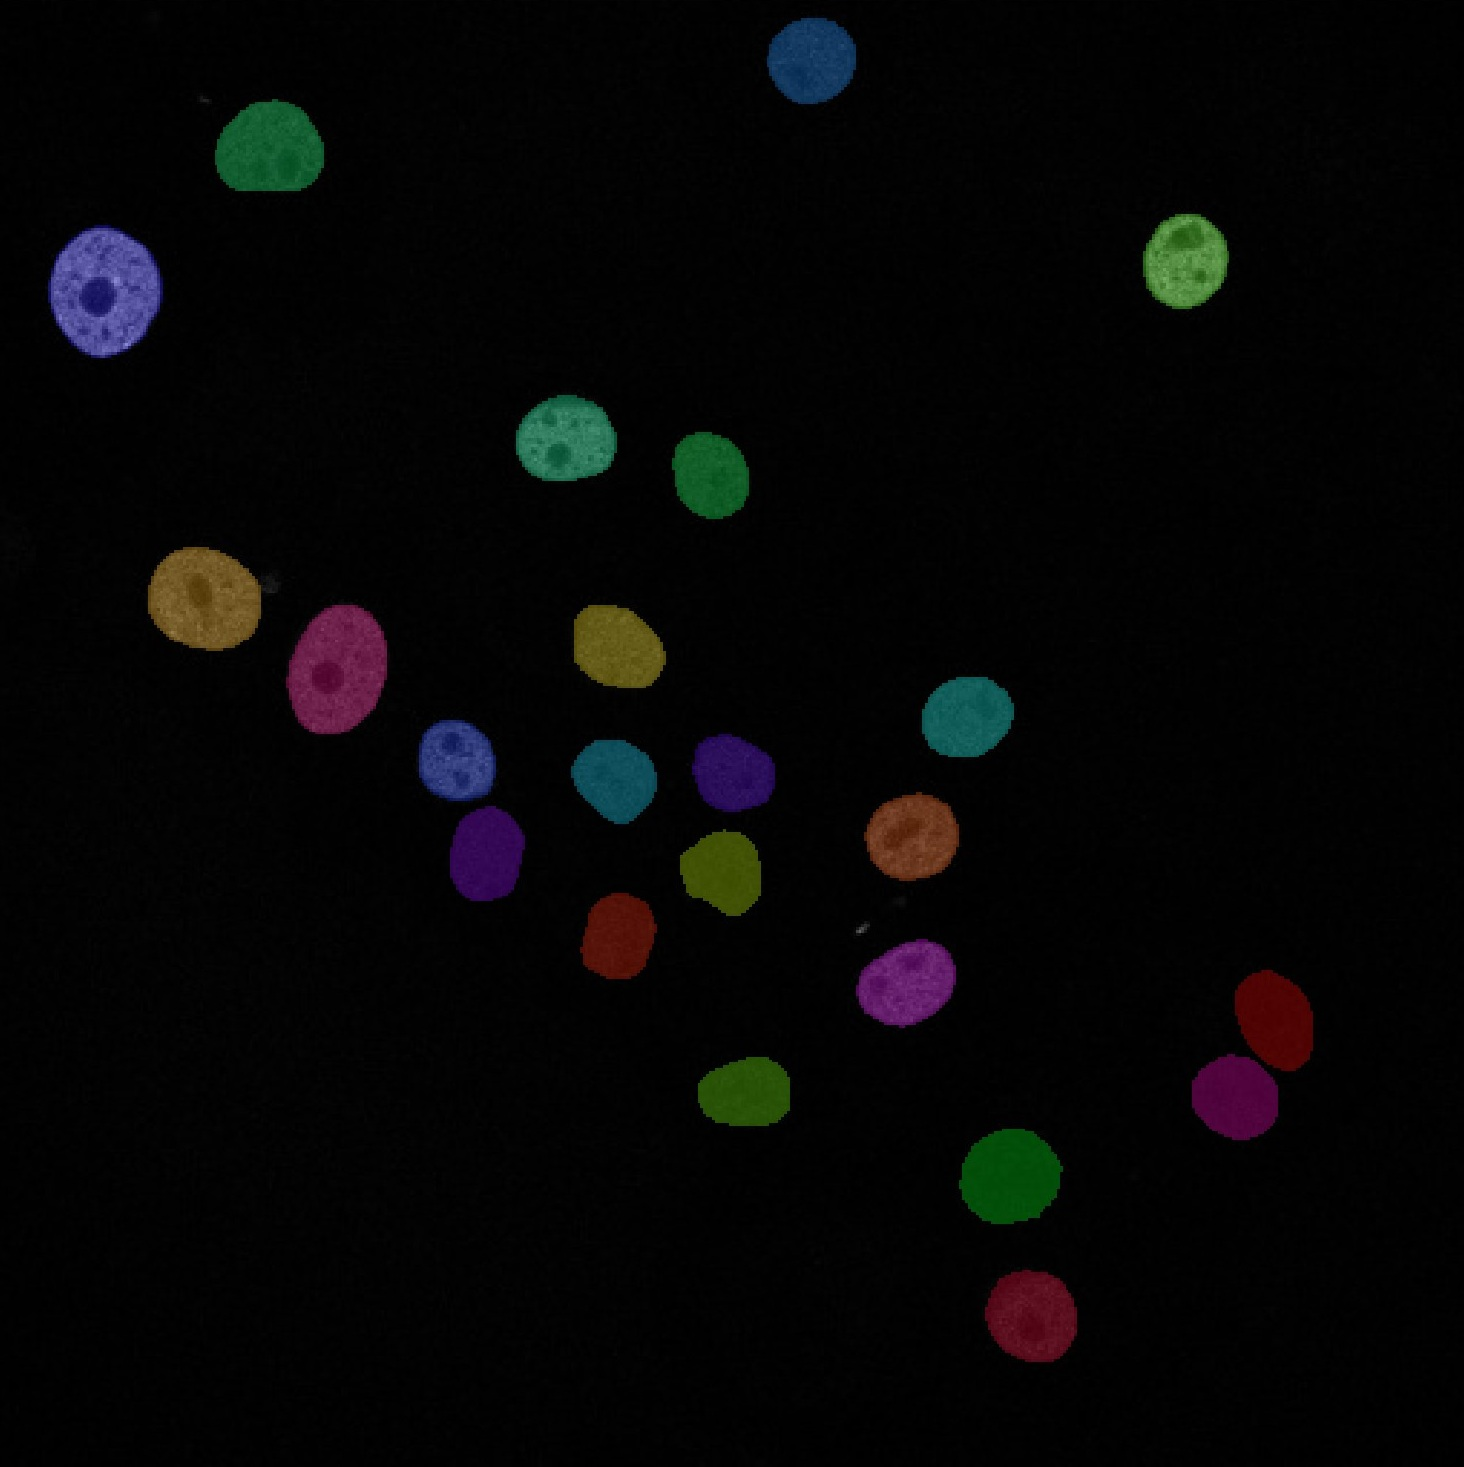
\includegraphics[width=\textwidth,height=3cm]{images/examples/gowt1_segmented.jpg}
    \caption{\footnotesize Fluo GOWT1}
    \label{fig:gowt1}
  \end{subfigure}
  \hfill
  \begin{subfigure}{0.23\textwidth}
    \centering
    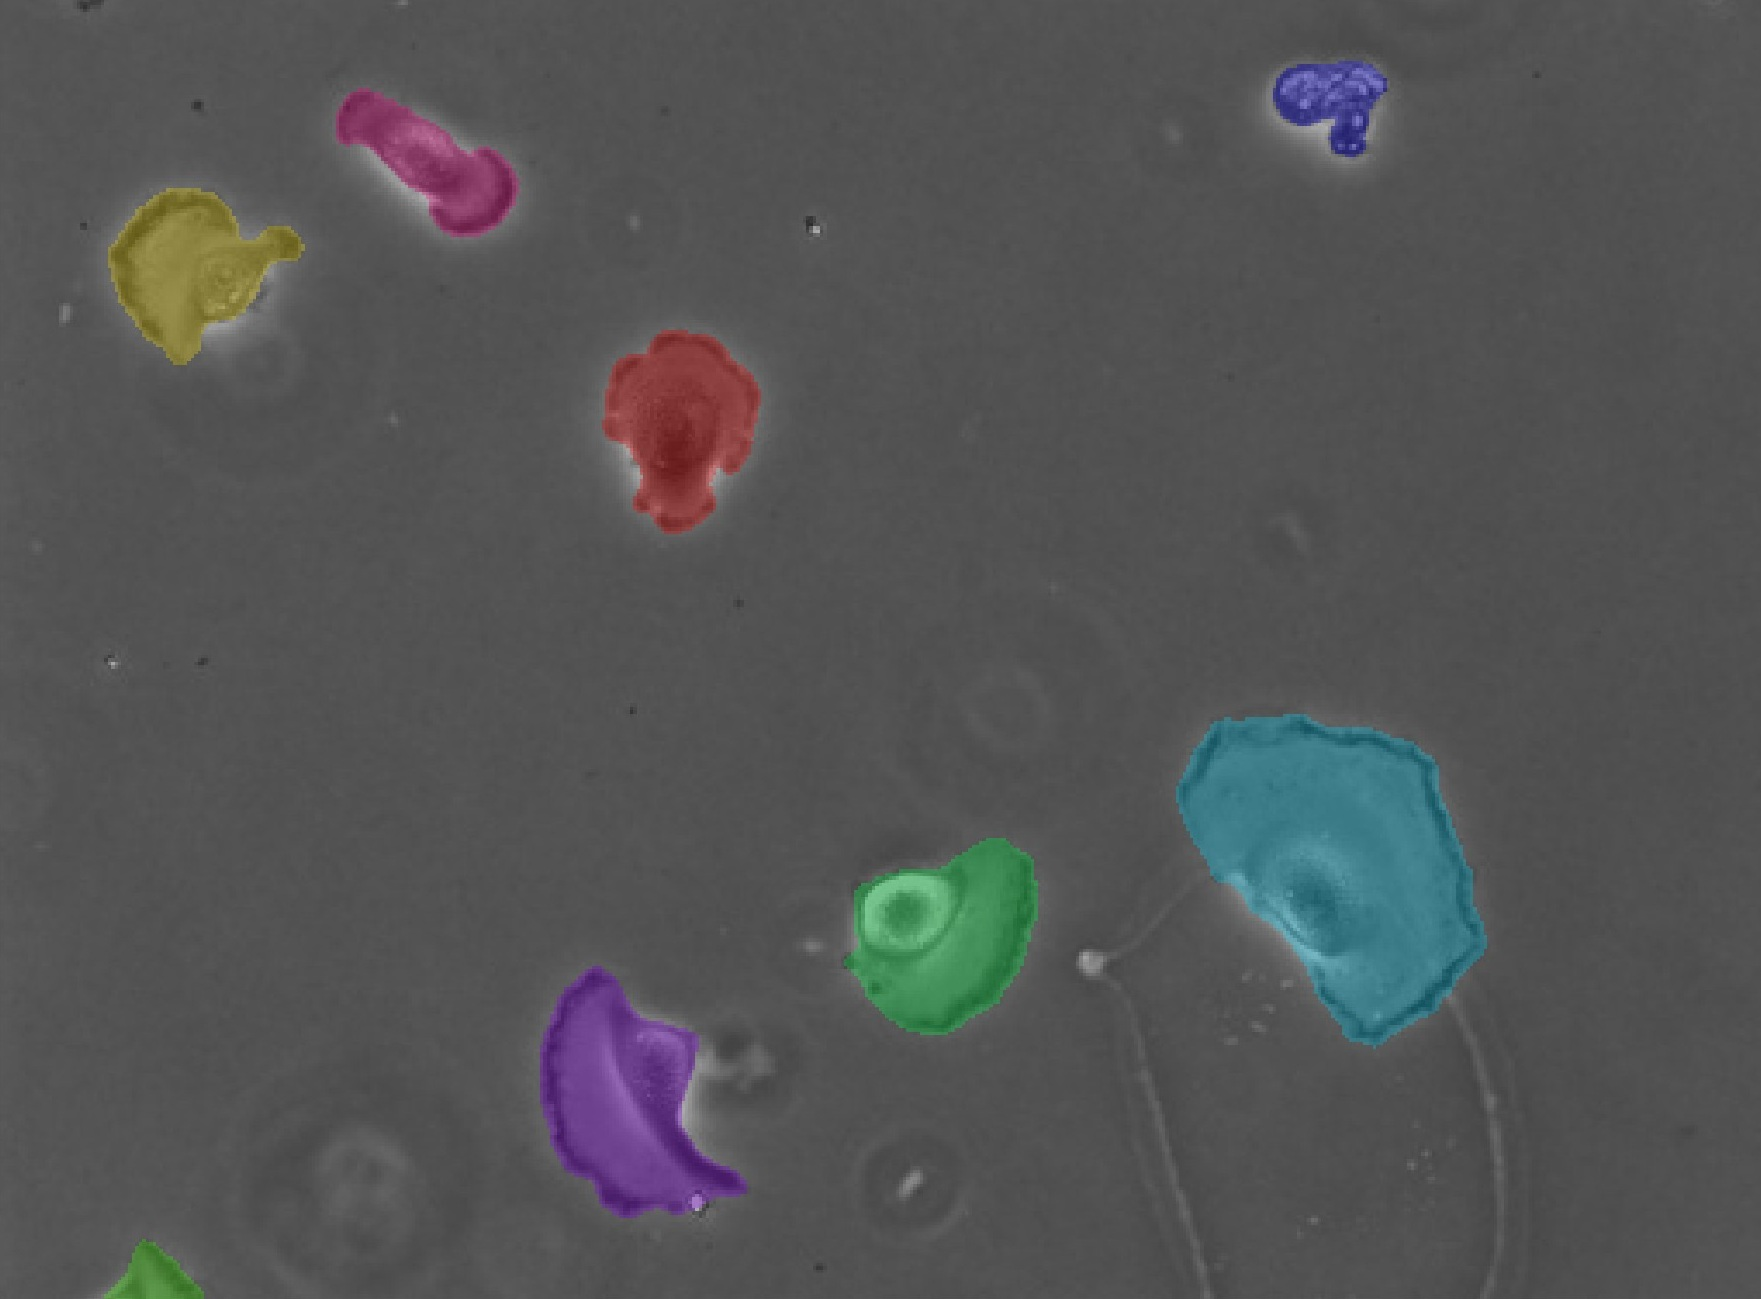
\includegraphics[width=\textwidth,height=3cm]{images/examples/u373_segmented.jpg}
    \caption{\footnotesize PhC U373}
    \label{fig:u373}
  \end{subfigure}
  \hfill
  \begin{subfigure}{0.23\textwidth}
    \centering
    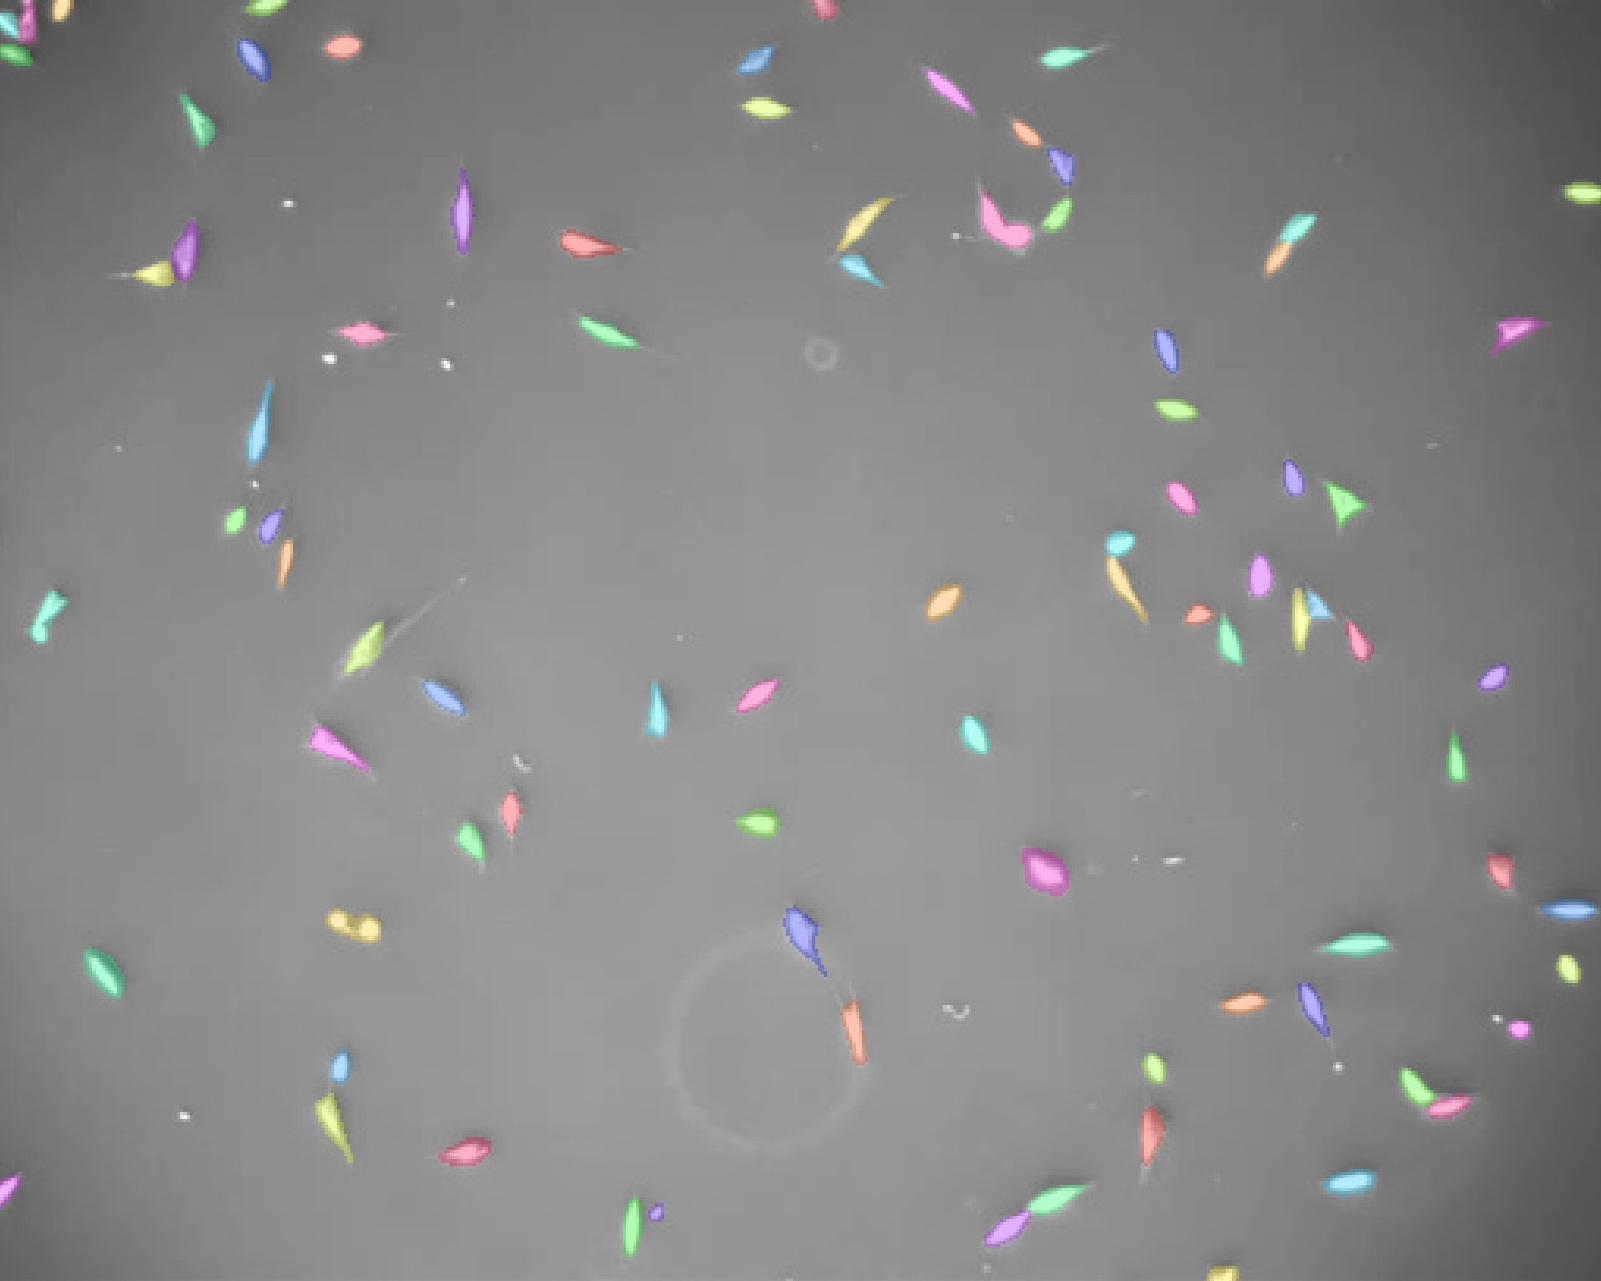
\includegraphics[width=\textwidth,height=3cm]{images/examples/psc_segmented.jpg}
    \caption{\footnotesize PhC PSC}
    \label{fig:psc}
  \end{subfigure}

  \caption{CellSeek segmentation results across diverse microscopy techniques and cell types. Microscopy images are shown with segmentation overlays demonstrating successful cell boundary detection across (top row) custom brightfield microscopy datasets including fibroblasts, 293T cells, MDA-MB-231 breast cancer cells, and COS-7 cells; (middle row) mixed imaging modalities including brightfield myosin imaging, brightfield hematopoietic stem cells (HSC), differential interference contrast (DIC) HeLa cells, and fluorescent Huh7 hepatocytes; (bottom row) fluorescent mesenchymal stem cells (MSC), GOWT1 mouse embryonic stem cells, and phase contrast U373 glioblastoma and pancreatic stellate cells (PSC). Examples include datasets from the Cell Tracking Challenge. The segmentation overlays demonstrate accurate cell boundary detection without parameter modifications or model retraining across these diverse imaging conditions.}
  \label{fig:generalization_examples}
\end{figure}

The examples span four major microscopy modalities: brightfield illumination (6 examples), fluorescence microscopy (3 examples), differential interference contrast (1 example), and phase contrast microscopy (2 examples). Cell types range from primary cells (fibroblasts, stem cells) to established cell lines (293T, HeLa, COS-7) and cancer cell lines (MDA-MB-231, U373), encompassing diverse morphologies, sizes, and optical properties. The segmentation overlays in each image demonstrate accurate cell boundary detection and successful adaptation to varying contrast conditions, cell densities, and morphological characteristics. This visual evidence supports CellSeek's foundation model integration providing robust performance across the spectrum of common cell biology applications without requiring specialized parameter tuning or domain-specific training.

\subsection{Generalization Across Imaging Modalities}

To validate our generalization capabilities beyond the examples shown in Figure \ref{fig:generalization_examples}, we conducted systematic testing across additional imaging conditions without parameter modification:

\textbf{Fluorescence Microscopy:} Successfully tracked nuclear markers (DAPI, H2B-GFP) and cytoplasmic labels (CellTracker, GFP) across multiple cell lines beyond those shown in the figure.

\textbf{Phase-Contrast:} Robust performance maintained across varying cell densities and morphological states, as demonstrated in the phase contrast examples.

\textbf{Brightfield:} Effective tracking of both bacterial colonies and mammalian cells in brightfield illumination, building on the diverse brightfield examples presented.

\textbf{Live-Cell Imaging:} Maintained tracking accuracy across multi-hour time-lapse sequences with cell divisions and morphological changes across all modalities tested.

The consistent performance across this broad range of imaging conditions, as exemplified in Figure \ref{fig:generalization_examples}, validates CellSeek's foundation model-based approach for achieving robust generalization without requiring modality-specific parameter optimization.

\subsection{Failure Mode Analysis}

CellSeek exhibits predictable failure modes that align with fundamental limitations of the underlying foundation models:

\begin{itemize}
  \item \textbf{Extreme Cell Density:} When cells are too densely packed for SAM to distinguish boundaries
  \item \textbf{Low Signal-to-Noise:} Very dim or noisy images that challenge even foundation model robustness
  \item \textbf{Rapid Morphological Changes:} Cells undergoing dramatic shape changes that exceed the adapted Cutie's last-frame temporal consistency assumptions
  \item \textbf{Complex Division Events:} Multi-daughter divisions or asymmetric divisions that violate tracking assumptions
\end{itemize}

Importantly, these limitations are clearly communicated through the GUI's confidence indicators, allowing users to identify problematic regions and apply targeted manual corrections using the intuitive SAM interface.

\end{document}
